\documentclass[tikz,border=12pt]{standalone}
\usepackage{amsmath,amssymb,amsfonts}
\usepackage{tikz}
\usetikzlibrary{shapes,arrows.meta,positioning,calc,fit,backgrounds,decorations.pathreplacing,shadows}

% --- Color Palette ---
\definecolor{themeblue}{RGB}{37, 99, 235}
\definecolor{themeteal}{RGB}{13, 148, 136}
\definecolor{themepurple}{RGB}{124, 58, 237}
\definecolor{themeorange}{RGB}{234, 88, 12}
\definecolor{themegreen}{RGB}{22, 163, 74}
\definecolor{themered}{RGB}{220, 38, 38}
\definecolor{themegray}{RGB}{100, 116, 139}
\definecolor{themecyan}{RGB}{6, 182, 212}
\definecolor{themeamber}{RGB}{217, 119, 6}

\begin{document}
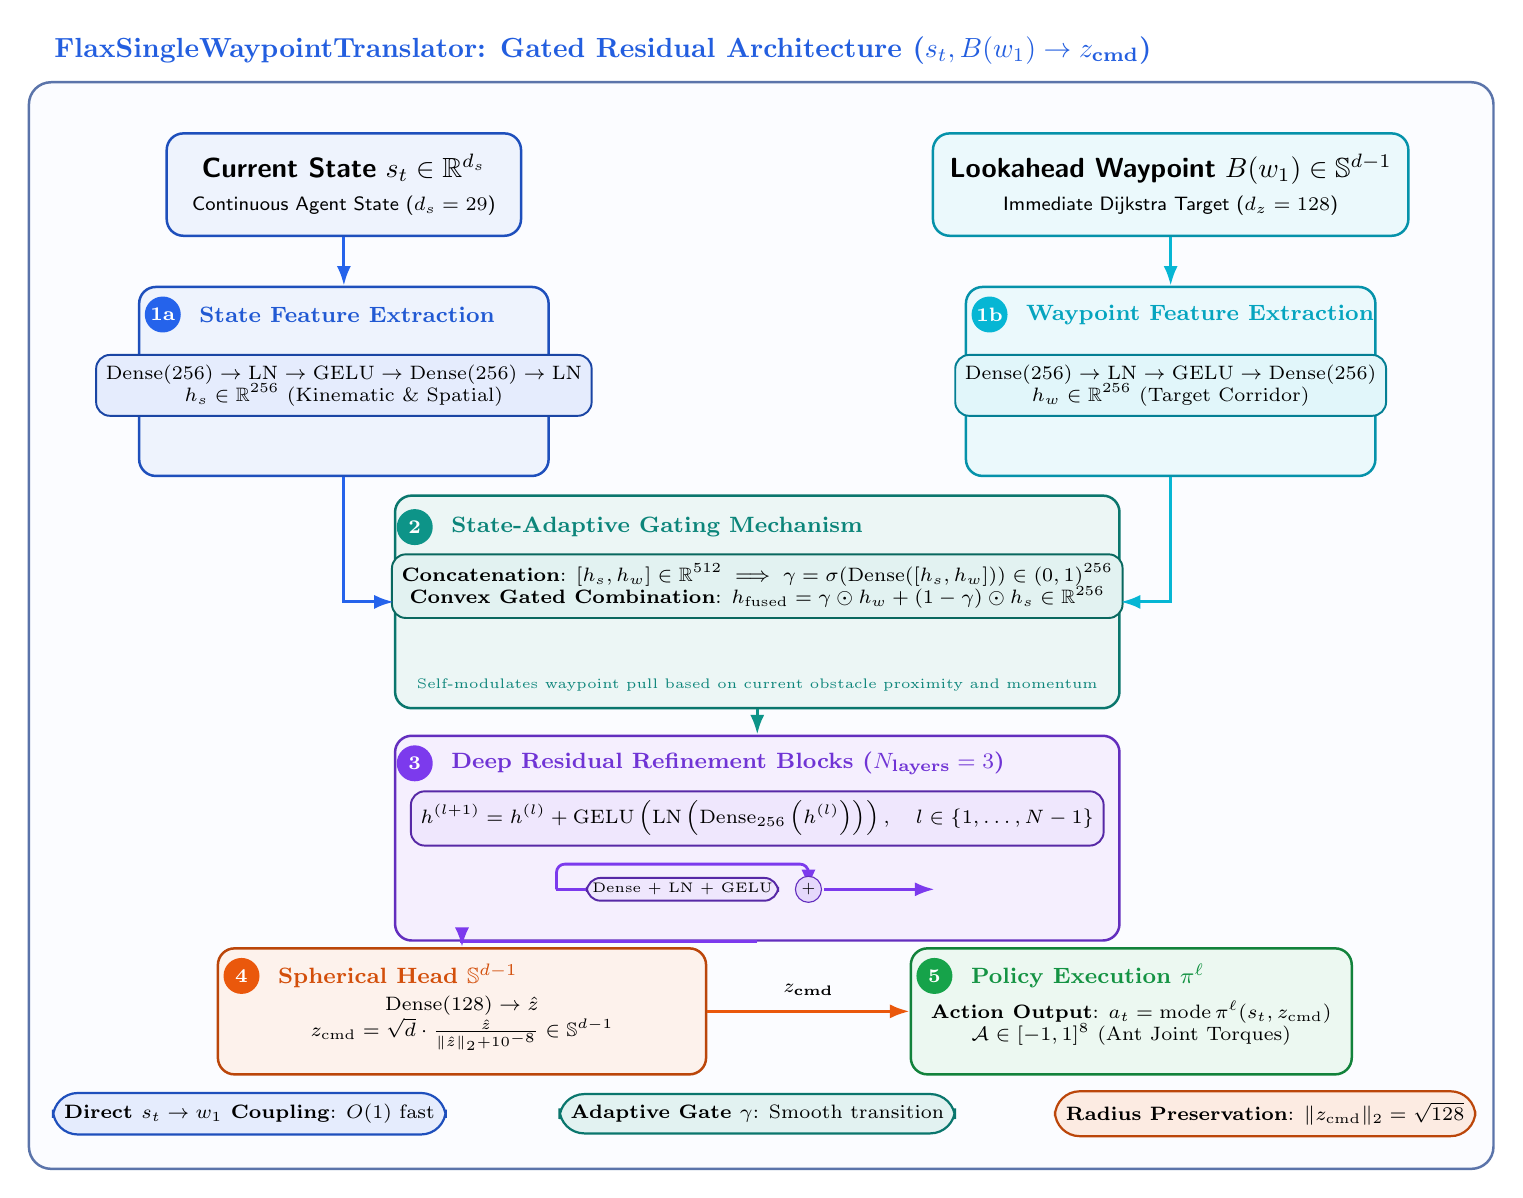
\begin{tikzpicture}[
    >=Latex,
    font=\sffamily,
    % Node styles
    box/.style={
        rectangle,
        rounded corners=6pt,
        draw=#1!80!black,
        fill=#1!8,
        line width=0.9pt,
        align=center,
        inner sep=6pt
    },
    subbox/.style={
        rectangle,
        rounded corners=5pt,
        draw=#1!70!black,
        fill=#1!12,
        line width=0.7pt,
        align=center,
        inner sep=3.5pt
    },
    badge/.style={
        circle,
        fill=#1,
        text=white,
        font=\bfseries\scriptsize,
        inner sep=0.5pt,
        minimum size=13pt
    },
    pill/.style={
        rectangle,
        rounded corners=9pt,
        draw=#1!80!black,
        fill=#1!12,
        line width=0.8pt,
        align=center,
        inner sep=4pt
    },
    arr/.style={
        -{Latex[length=2.5mm,width=1.8mm]},
        line width=1.1pt,
        draw=themegray!80!black
    },
    carr/.style={
        -{Latex[length=2.5mm,width=1.8mm]},
        line width=1.1pt,
        draw=#1
    },
    darr/.style={
        -{Latex[length=2.3mm,width=1.6mm]},
        line width=1.0pt,
        dashed,
        draw=#1
    }
]

% ==============================================================================
% TITLE
% ==============================================================================
\node[anchor=west, font=\bfseries\normalsize, text=themeblue!95!black] at (-0.3, 8.4) 
    {FlaxSingleWaypointTranslator: Gated Residual Architecture ($s_t, B(w_1) \to z_{\text{cmd}}$)};

% Main Enclosing Canvas
\draw[rounded corners=8pt, line width=0.9pt, draw=themeblue!40!gray, fill=themeblue!2] 
    (-0.5, -5.8) rectangle (18.1, 8.0);

% ==============================================================================
% 1. INPUT LAYER
% ==============================================================================
\node[box=themeblue, minimum width=4.5cm, minimum height=1.3cm] (in_state) at (3.5, 6.7) 
    {\textbf{Current State} $s_t \in \mathbb{R}^{d_s}$\\\scriptsize Continuous Agent State ($d_s=29$)};

\node[box=themecyan, minimum width=4.5cm, minimum height=1.3cm] (in_wp) at (14.0, 6.7) 
    {\textbf{Lookahead Waypoint} $B(w_1) \in \mathbb{S}^{d-1}$\\\scriptsize Immediate Dijkstra Target ($d_z=128$)};

% ==============================================================================
% 2. DUAL FEATURE EXTRACTION ENCODERS (STEP 1)
% ==============================================================================
% State Branch
\node[box=themeblue, minimum width=5.2cm, minimum height=2.4cm] (enc_s) at (3.5, 4.2) {};
\node[badge=themeblue] (b1_s) at (1.2, 5.05) {1a};
\node[font=\bfseries\footnotesize, text=themeblue!90!black, right=3pt of b1_s] {State Feature Extraction};
\node[subbox=themeblue, font=\scriptsize, minimum width=4.6cm] at (3.5, 4.15) 
    {$\text{Dense}(256) \to \text{LN} \to \text{GELU} \to \text{Dense}(256) \to \text{LN}$\\
    $h_s \in \mathbb{R}^{256}$ (Kinematic \& Spatial)};

% Waypoint Branch
\node[box=themecyan, minimum width=5.2cm, minimum height=2.4cm] (enc_w) at (14.0, 4.2) {};
\node[badge=themecyan] (b1_w) at (11.7, 5.05) {1b};
\node[font=\bfseries\footnotesize, text=themecyan!90!black, right=3pt of b1_w] {Waypoint Feature Extraction};
\node[subbox=themecyan, font=\scriptsize, minimum width=4.6cm] at (14.0, 4.15) 
    {$\text{Dense}(256) \to \text{LN} \to \text{GELU} \to \text{Dense}(256)$\\
    $h_w \in \mathbb{R}^{256}$ (Target Corridor)};

\draw[carr=themeblue] (in_state) -- (enc_s);
\draw[carr=themecyan] (in_wp) -- (enc_w);

% ==============================================================================
% 3. GATING MECHANISM & FUSION (STEP 2)
% ==============================================================================
\node[box=themeteal, minimum width=9.2cm, minimum height=2.7cm] (gate_box) at (8.75, 1.4) {};
\node[badge=themeteal] (b2) at (4.4, 2.35) {2};
\node[font=\bfseries\footnotesize, text=themeteal!90!black, right=3pt of b2] {State-Adaptive Gating Mechanism};

\node[subbox=themeteal, font=\scriptsize, minimum width=8.6cm] at (8.75, 1.6) 
    {\textbf{Concatenation}: $[h_s, h_w] \in \mathbb{R}^{512} \implies \gamma = \sigma(\text{Dense}( [h_s, h_w] )) \in (0, 1)^{256}$\\
    \textbf{Convex Gated Combination}: $h_{\text{fused}} = \gamma \odot h_w + (1 - \gamma) \odot h_s \in \mathbb{R}^{256}$};
\node[font=\tiny, text=themeteal!90!black] at (8.75, 0.35) {Self-modulates waypoint pull based on current obstacle proximity and momentum};

\draw[carr=themeblue] (enc_s.south) |- (gate_box.west);
\draw[carr=themecyan] (enc_w.south) |- (gate_box.east);

% ==============================================================================
% 4. DEEP RESIDUAL REFINEMENT BLOCKS (STEP 3)
% ==============================================================================
\node[box=themepurple, minimum width=9.2cm, minimum height=2.6cm] (res_box) at (8.75, -1.6) {};
\node[badge=themepurple] (b3) at (4.4, -0.65) {3};
\node[font=\bfseries\footnotesize, text=themepurple!90!black, right=3pt of b3] {Deep Residual Refinement Blocks ($N_{\text{layers}}=3$)};

\node[subbox=themepurple, font=\scriptsize, minimum width=8.6cm] at (8.75, -1.35) 
    {$h^{(l+1)} = h^{(l)} + \text{GELU}\left(\text{LN}\left(\text{Dense}_{256}\left(h^{(l)}\right)\right)\right), \quad l \in \{1, \dots, N-1\}$};

% Skip Connection Illustration Inside ResBox
\begin{scope}[shift={(6.2, -2.25)}]
    \draw[carr=themepurple, line width=1.0pt] (0, 0) -- (1.3, 0);
    \draw[rounded corners=3pt, carr=themepurple, line width=1.0pt] (0, 0) -- ++(0, 0.32) -- ++(3.2, 0) -- ++(0, -0.32);
    \node[circle, draw=themepurple!80!black, fill=themepurple!20, inner sep=1pt, font=\tiny\bfseries] at (3.2, 0) {$+$};
    \node[subbox=themepurple, font=\tiny, inner sep=2pt] at (1.6, 0) {Dense + LN + GELU};
    \draw[carr=themepurple, line width=1.0pt] (3.4, 0) -- (4.8, 0);
\end{scope}

\draw[carr=themeteal] (gate_box.south) -- (res_box.north);

% ==============================================================================
% 5. SPHERICAL PROJECTION & LOW-LEVEL POLICY (STEPS 4 & 5)
% ==============================================================================
% Spherical Head
\node[box=themeorange, minimum width=6.2cm, minimum height=1.6cm] (sphere_head) at (5.0, -3.8) {};
\node[badge=themeorange] (b4) at (2.2, -3.35) {4};
\node[font=\bfseries\footnotesize, text=themeorange!90!black, right=3pt of b4] {Spherical Head $\mathbb{S}^{d-1}$};
\node[font=\scriptsize, align=center] at (5.0, -3.95) 
    {$\text{Dense}(128) \to \hat{z}$\\$z_{\text{cmd}} = \sqrt{d} \cdot \frac{\hat{z}}{\|\hat{z}\|_2 + 10^{-8}} \in \mathbb{S}^{d-1}$};

% Low-Level Policy Execution
\node[box=themegreen, minimum width=5.6cm, minimum height=1.6cm] (low_policy) at (13.5, -3.8) {};
\node[badge=themegreen] (b5) at (11.0, -3.35) {5};
\node[font=\bfseries\footnotesize, text=themegreen!90!black, right=3pt of b5] {Policy Execution $\pi^\ell$};
\node[font=\scriptsize, align=center] at (13.5, -3.95) 
    {\textbf{Action Output}: $a_t = \operatorname{mode}\pi^\ell(s_t, z_{\text{cmd}})$\\
    $\mathcal{A} \in [-1, 1]^8$ (Ant Joint Torques)};

\draw[carr=themepurple] (res_box.south) -| (sphere_head.north);
\draw[carr=themeorange] (sphere_head.east) -- node[above=2pt, font=\scriptsize\bfseries] {$z_{\text{cmd}}$} (low_policy.west);


% ==============================================================================
% BOTTOM SUMMARY PILLS
% ==============================================================================
\node[pill=themeblue, font=\scriptsize, minimum width=4.9cm] at (2.3, -5.1) 
    {\textbf{Direct $s_t \to w_1$ Coupling}: $O(1)$ fast};

\node[pill=themeteal, font=\scriptsize, minimum width=4.9cm] at (8.75, -5.1) 
    {\textbf{Adaptive Gate $\gamma$}: Smooth transition};

\node[pill=themeorange, font=\scriptsize, minimum width=4.9cm] at (15.2, -5.1) 
    {\textbf{Radius Preservation}: $\|z_{\text{cmd}}\|_2 = \sqrt{128}$};

\end{tikzpicture}
\end{document}
